\documentclass[a4paper]{article}
\usepackage[left=3cm,right=3cm,top=2cm,bottom=2cm]{geometry} % page settings
\usepackage{enumerate}
\usepackage{enumitem}
\usepackage{hyperref}
\usepackage{graphicx}
\usepackage{amsfonts}
\usepackage{verbatim}
\usepackage{amsthm}
\usepackage{amssymb}
\usepackage{mathtools}
\usepackage{wasysym}
\usepackage{xspace}
\usepackage{xpatch}
\usepackage{titlesec}
\usepackage{polski}
\usepackage{tikz}
\usepackage[utf8]{inputenc}
\titlespacing*{\subsection}
{0ex}{10ex}{3ex}

\author{Kamil Matuszewski 272331}
\title{\textbf{Bazy danych} \\ System wspomagający organizację konferencji}
\begin{document}
\maketitle

\section{Model konceptualny}
Obrazek przedstawiający model konceptualny można znaleźć na następnej stronie. Mamy osiem encji:
\begin{itemize}
\item \textbf{uczestnik(login,haslo,uprawnienia)} - Przechowuje informacje o uczestnikach a także o organizatorach (opis ról poniżej). Login jest unikalnym identyfikatorem.
\item \textbf{wydarzenie(nazwa,start,koniec)} - Przechowuje informacje o wydarzeniach - nazwa jest unikalnym identyfikatorem, a start i koniec to kolejno data początku i końca wydarzenia.
\item \textbf{referat(id,prowadzacy,tytul,poczatek,pokoj,wydarzenie,status)} - Przechowuje informacje o kolejnych referatach. Id jest unikalnym identyfikatorem. Referat może nie należeć do żadnego wydarzenia, ale jeśli należy, to czas rozpoczęcia musi być z przedziału [początek,koniec] odpowiadającego mu wydarzenia. Jeśli status jest równy p, to poczatek, pokoj i wydarzenie są nullami. Status d jest używany tylko do usuwania krotki, w przeciwnym wypadku przy usuwaniu zmieniamy status na "u".
\item \textbf{propozycja\_znajomosci(login\_1,login\_2)} - Przechowuje informacje o propozycjach znajomości, jeśli propozycja jest symetryczna to odpowiednie krotki są usuwane, a informacja o znajomości dodawana jest do tabeli \textbf{zna}. Oba atrybuty są kluczami obcymi odnoszącymi się do encji \textbf{uczestnik}.
\item \textbf{zna(login\_1,login\_2)} - Informacja mówiąca, że użytkownik login\_1 zna użytkownika login\_2, znajomość jest symetryczna. Oba atrybuty są kluczami obcymi odnoszącymi się do encji \textbf{uczestnik}.
\item \textbf{zarejestrowal\_sie(login\_uczestnika,nazwa\_wydarzenia)} - Informacja o tym, że użytkownik zarejestrował się na dane wydarzenie. Pierwszy atrybut jest kluczem obcym wskazującym na encję \textbf{uczestnik}, drugi jest kluczem obcym wskazującym na encję \textbf{wydarzenie}.
\item \textbf{uczestniczyl(login\_uczestnika,id\_referatu)} - Informacja o tym, że użytkownik uczestniczył w referacie (odnotowana jest faktyczna obecność). Pierwszy atrybut jest kluczem obcym wskazującym na encję \textbf{uczestnik}, drugi jest kluczem obcym wskazującym na encję \textbf{referat}.
\item \textbf{ocenil(login\_uczestnika,id\_referatu,ocena)} - Informacja o ocenie danego referatu przez danego użytkownika. Pierwszy atrybut jest kluczem obcym wskazującym na encję \textbf{uczestnik}, drugi jest kluczem obcym wskazującym na encję \textbf{referat}, trzeci jest oceną referatu w skali 1-10.

\end{itemize}


\centerline{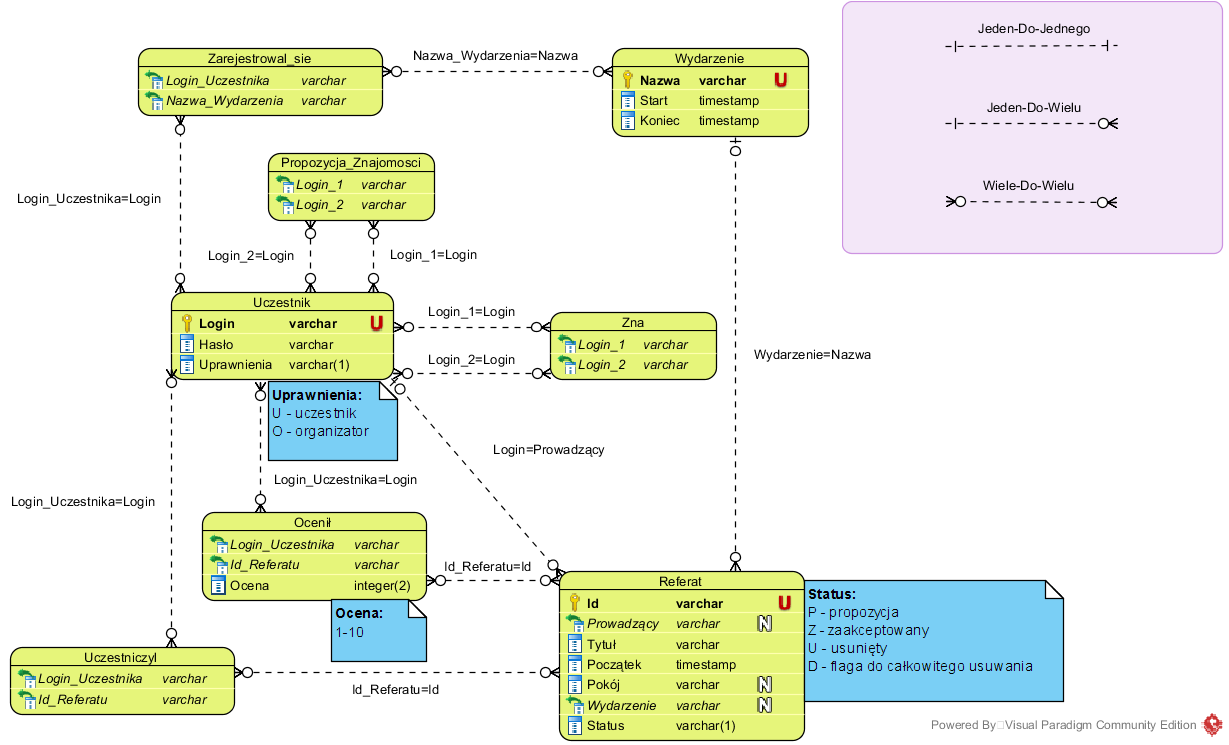
\includegraphics[angle=90,scale=1]{konceptualny.png}}


\subsection{Opis ról}
Mimo, że nie ma określonych ról w samej bazie, to dostęp do niektórych funkcji wymaga podania loginu i hasła. Login i hasło są następnie sprawdzane w bazie, i zwracana jest rola użytkownika i sprawdzane są uprawnienia do wykonania podanej funkcji. Wyróżniamy więc role:
\begin{itemize}
\item Uczestnik - osoba która w bazie ma status uczestnika ma dostęp do funkcji oznaczonych w specyfikacji przez "U". Tą rolę otrzymuje każdy nowy użytkownik stworzony za pomocą polecenia \textit{user}.
\item Organizator - osoba która w bazie ma status organizatora ma dostęp do funkcji oznaczonych w specyfikacji przez "O". Tę rolę otrzymują użytkownicy stworzeni za pomocą polecenia \textit{organizer}. W szczególności organizator nie jest rozszerzeniem uprawnień uczestnika (nie ma dostępu do funkcji oznaczonych w specyfikacji przez "U").	\end{itemize}

\section{Model fizyczny}
Model fizyczny wraz z odpowiednimi komentarzami znajduje się w pliku \textbf{fizyczny.sql}. Funkcje są odpowiednio ponazywane a także posiadają komentarze mówiące, do którego z zapytań się odnoszą. Do tego utworzone zostały odpowiednie typy, by funkcje mogły zwrócić odpowiednio przemianowane krotki (dla ułatwienia działania aplikacji).

\section{Aplikacja}
Aplikacja okienkowa napisana jest w technologii .NET Core. Użyte biblioteki:
\begin{itemize}
\item \textit{Npgsql} - biblioteka do łączenia się z bazą danych.
\item \textit{Newtonsoft.Json} - biblioteka do przetwarzania zapytań Json a także do tworzenia obiektów wynikowych.
\item \textit{Dapper} - biblioteka do wykonywania zapytań a także do zbierania wyników.
\end{itemize}

\subsection{Działanie aplikacji}
Podczas każdego uruchomienia, program czyta pierwszą linię i (zgodnie ze specyfikacją) traktuje ją jak Jsonowe zapytanie "open". Zapytanie to otwiera bazę danych, tworząc nowy obiekt \textit{Database}. Obiekt ten przechowuje wszystkie potrzebne informacje, zawiera też metody umożliwiające wykonywanie poszczególnych zapytań do bazy danych. Jeśli otwarta baza nie zawiera tabeli "uczestnik", to znaczy, że jest pusta (zgodnie ze specyfikacją), wczytujemy więc model fizyczny z pliku \textbf{fizyczny.sql}.

Jeśli wszystko było w porządku, to w pętli wczytujemy i przetwarzamy kolejne linie. Poszczególne odpowiedzi wrzucamy na kolejkę, by następnie wypisać wszystkie zapytania pod koniec działania programu.

Każde zapytanie jest odpowiednio przetwarzane w celu zdobycia nazwy funkcji a także wszystkich potrzebnych danych a następnie umieszczone w obiekcie \textbf{Input}. Wywoływana jest odpowiednia funkcję i po wykonaniu zapytania do bazy danych zwracamy obiekt typu \textit{Output} zawierający status (\textit{OK/ERROR/NOT IMPLEMENTED}) oraz wynik zapytania jeśli jest to wymagane. Następnie z obiektu tworzony jest Json, który wrzucany jest na kolejkę.

Aplikacja odpowiada jedynie za przetwarzanie obiektów Json i komunikacji pomiędzy użytkownikiem a bazą danych. O wszystkie zapytania dbają odpowiednie funkcje opisane w modelu fizycznym. Oznacza to, że przy zmianie modelu fizycznego nie trzeba niczego zmieniać w aplikacji, dopóki odpowiednie funkcje będą miały te same nazwy, argumenty i zwracały te same wartości. Aplikacja jest zabezpieczona przed tzw. \textbf{SQL injection} o co dba biblioteka \textit{Dapper}.

Obiekt \textit{Data} zawiera dane wynikowe, wczytane wprost z bazy danych. Z uwagi na to, że w jednym z zapytań argument wyjściowy musi być nazwany "event" a nazwanie w ten sposób zmiennej jest niemożliwe, zmienna jest nazwana "\_event" i dopiero podczas przetwarzania obiektu do Jsona jej nazwa jest odpowiednio zmieniana.

Po przetworzeniu zapytań i wypisaniu odpowiedzi aplikacja kończy działanie.

\section{Włączanie aplikacji}
Aplikacja do uruchomienia wymaga zainstalowanego .NET Core, a do poprawnego działania wymaga także postgresa i pustej bądź wypełnionej zgodnie z modelem fizycznym bazy danych.

\subsection{Instalacja .NET Core}
Instalacja .NET Core przebiega zgodnie z instrukcją opisaną na stronie \url{https://www.microsoft.com/net/core}. Z uwagi na dostęp do tej instrukcji a także przez nieznajomość systemu użytkownika, nie będę opisywać kolejnych kroków instalacyjnych.

\subsection{Uruchomienie}
Kiedy znajdujemy się w folderze głównym projektu, podczas pierwszego uruchomienia należy najpierw wpisać polecenie \textbf{dotnet restore}, żeby pozyskać wszystkie biblioteki niezbędne do uruchomienia. By uruchomić samą aplikację należy wpisać \textbf{dotnet run}.

\section{Testy}
W pliku \textit{test} znajdują się wygenerowane przeze mnie testy. Generują one niedużą bazę danych, która służyła mi za obiekt testów. Linijka 1 odpowiada za połączenie się z bazą danych (należy ją odpowiednio uzupełnić), od 2 do 1013 (włącznie) są operacje modyfikujące bazę danych. Linijki 1014-1026 to przykładowe zapytania zwracające dane. W testach nie zostały ujęte wszystkie możliwości a także nie zostały sprawdzone wszystkie przypadki brzegowe - służą one jedynie do upewnienia się, że aplikacja rzeczywiście potrafi się komunikować z bazą danych. 

\end{document}
